%%%%%%%%%%%%%%%%%%%%%%%%%%%%%%%%%%%%%%%%%%%%%%%%%%%%%%%%%%%%%%%%%%%%%%%%%%%%%%%
\section{Comprensión del problema y de los datos}
\label{sec:comprension}
%%%%%%%%%%%%%%%%%%%%%%%%%%%%%%%%%%%%%%%%%%%%%%%%%%%%%%%%%%%%%%%%%%%%%%%%%%%%%%%

Este capítulo y los siguientes describen el desarrollo del proyecto de acuerdo con las fases de la metodología CRISP-ML. En este primer capítulo se aborda la comprensión de los datos: se revisan los conjuntos de datos disponibles para la tarea de texto a pictogramas, se explica la elección del corpus con el que se entrenará el modelo y se describe la fuente del vocabulario de pictogramas, el catálogo de ARASAAC, junto con la forma en que se consulta a través de su API (\textit{Application Programming Interface}, interfaz de programación de aplicaciones).

\subsection{Conjunto de datos de ToPicto}
El primer conjunto de datos que se analizó es el que proporciona CLEF (\textit{Conference and Labs of the Evaluation Forum}) para la tarea de traducción a pictogramas. Su análisis permitió identificar una característica importante. Sus datos provienen de los corpus Propicto \cite{macaire2024}, cuyas secuencias de pictogramas se generaron con un conjunto de reglas, y solo una fracción muy pequeña fue revisada por personas: en \textit{Propicto-Orfeo}, 1,200 de cerca de 290 mil enunciados.
Al final del proceso, los lemas se asocian con los identificadores de los pictogramas. El flujo completo se muestra en la Figura~\ref{fig:propicto_pipeline}.

\begin{figure}[H]
    \centering
    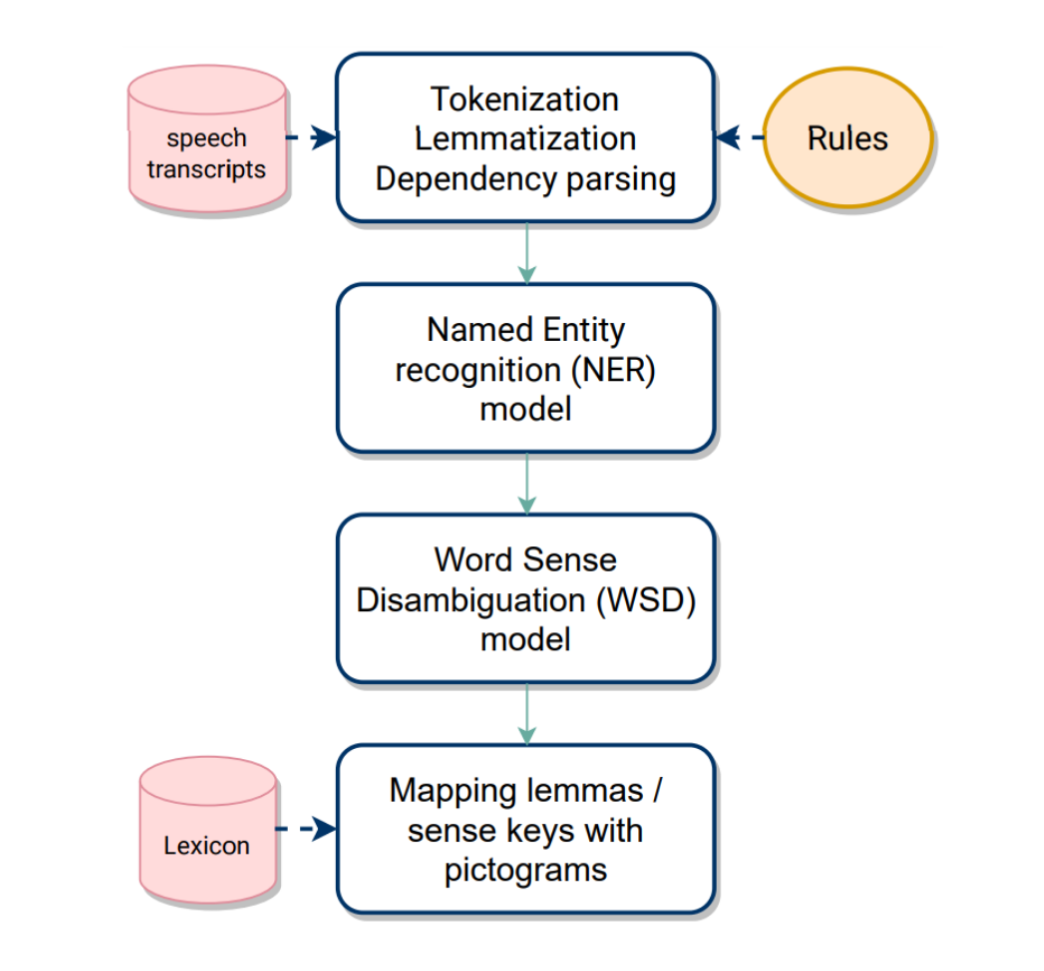
\includegraphics[width=0.45\textwidth]{img/propicto orfeo pipeline.png}
    \caption{Flujo seguido para crear los corpus Propicto, descrito para \textit{Propicto-Orfeo} \cite{macaire2024propicto}; \textit{Propicto-CommonVoice} se generó con el mismo formalismo de reglas. Las oraciones de ejemplo representadas en pictogramas se obtuvieron mediante traducción automática.}
    \label{fig:propicto_pipeline}
\end{figure}
% VERIFICAR: en el documento se usan dos keys distintas, macaire2024 y macaire2024propicto. Unificar.

Esta característica tiene una consecuencia directa: si un modelo solo aprende la relación entre un texto y su secuencia de pictogramas, y esa secuencia se obtuvo con reglas fijas, su desempeño queda limitado por esas mismas reglas. Lo ideal sería que el modelo aprendiera un idioma nuevo: el de los pictogramas o, en su defecto, el de sus identificadores.

\subsection{Alternativa explorada: xP3mt}
Para enseñar un idioma nuevo a un modelo de lenguaje se revisó el trabajo ConlangBench \citep{jeong_conlangbench_2026}, en el que se ajustan modelos de lenguaje con LoRA para traducir, en ambas direcciones, entre el inglés y lenguas ficticias como el élfico. Sus resultados muestran que los modelos se apoyan en el conocimiento de los idiomas naturales que adquirieron durante el preentrenamiento. A partir de esta idea se exploró ir más allá de la traducción: entrenar con instrucciones variadas (resumir, ampliar textos, responder preguntas, clasificar o predecir), de modo que el modelo usara el nuevo lenguaje desde distintos enfoques en lugar de memorizar una correspondencia. Este planteamiento se inspira en el ajuste multitarea, que mejora la capacidad de los modelos para generalizar a tareas e idiomas nuevos \cite{muennighoff2022crosslingual}.

Con esta idea se consideró el conjunto de datos xP3mt \cite{muennighoff2022crosslingual}, creado por BigScience. Es una variante de xP3 (\textit{Crosslingual Public Pool of Prompts}), una colección de tareas de PLN (preguntas y respuestas, resumen, inferencia, paráfrasis, traducción, entre otras) en formato instrucción--respuesta, en 46 idiomas. En xP3mt las instrucciones se tradujeron automáticamente al idioma de cada ejemplo. El conjunto está disponible en Hugging Face (\texttt{bigscience/xP3mt}); la configuración en español tiene alrededor de 3.37 millones de registros con dos campos: \texttt{inputs} y \texttt{targets}.

La propuesta era aplicar las reglas de \textit{Propicto} solo a la columna \texttt{targets}. Así el modelo aprendería a responder instrucciones con secuencias de pictogramas.

Las pruebas con xP3mt orientaron la elección hacia un corpus diseñado específicamente para pictogramas. Las salidas de xP3mt son largas y complejas, como muestra la Tabla~\ref{tab:ejemplos_xp3mt}, y muchas de sus palabras no tienen un pictograma equivalente en ARASAAC, por lo que aprovecharlo requeriría validar manualmente cada traducción. Por ello se optó por un corpus cuyas secuencias ya están asociadas a pictogramas, como se describe a continuación.

\begin{table}[htbp]
    \centering
    \small
    \caption{Ejemplos del subconjunto en español de xP3mt. Los textos largos se recortaron con [\dots].}
    \label{tab:ejemplos_xp3mt}
    \begin{tabularx}{\textwidth}{>{\raggedright\arraybackslash}X >{\raggedright\arraybackslash}X}
        \toprule
        \textbf{inputs} & \textbf{targets} \\
        \midrule
        Crea la carpeta que quieras sincronizar, si es necesario. Abre el menú Inicio. Abre el Explorador de archivos. [\dots] I'm interested in that, but I only have a few mins. Can you give me at most the first 500 characters of a detailed explanation in Spanish about that?
        & Si quieres sincronizar una nueva carpeta en vez de hacerlo con una que ya existe, crea la carpeta siguiendo estos pasos: Ve a la ubicación donde quieras crear la carpeta (por ejemplo, el Escritorio). Haz clic derecho en un espacio en blanco. Selecciona Nuevo. [\dots] \\
        \midrule
        Mu mutima gw'olunaku, abatambuze balaba ebifaanani ebyamazzi nga balowooza nti mazzi (oba ebintu ebirala). The previous text is in Ganda. Here is a translation to Spanish:
        & Durante el calor diurno, es posible que los turistas vean espejismos que generan la ilusión de visualizar agua, entre otros. \\
        \midrule
        {}[Texto en hindi con instrucciones para obtener un recibo de Uber] Write a summary of the previous text in Spanish:
        & Ve a https://riders.uber.com en un navegador web. Inicia sesión en Uber. Haz clic en Mis viajes. Selecciona un viaje. Haz clic en Reenviar. \\
        \bottomrule
    \end{tabularx}
\end{table}

\subsection{Conjunto de datos elegido: Propicto-CommonVoice}
La familia de corpus Propicto incluye dos conjuntos en francés construidos con el mismo formalismo de reglas y el mismo vocabulario de ARASAAC \cite{macaire2024, propicto_commonvoice}. \textit{Propicto-Orfeo} contiene cerca de 290 mil enunciados de habla espontánea, es decir, conversaciones reales transcritas. \textit{Propicto-CommonVoice}, construido a partir de la versión 15.0 del corpus Common Voice en francés, contiene cerca de 560 mil enunciados de habla leída: personas que leen en voz alta oraciones escritas \cite{propicto_commonvoice}.

Se decidió usar \textit{Propicto-CommonVoice} por dos razones. Primero, es casi el doble de grande: su partición de entrenamiento tiene 527,554 registros, frente a 231,374 de \textit{Propicto-Orfeo}. Segundo, sus oraciones están escritas y bien formadas, sin titubeos ni repeticiones, por lo que se parecen más a la entrada que recibirá el modelo, ya que el usuario escribe el texto que desea traducir. El corpus mantiene sus particiones originales de entrenamiento, validación y prueba (527,554, 16,132 y 16,132 registros). Cada registro tiene cuatro campos: el identificador del audio (\texttt{clips}), el texto fuente (\texttt{text}), la lista de identificadores de pictograma (\texttt{pictos}) y las palabras clave en francés asociadas a cada pictograma (\texttt{tokens}). En este trabajo se usan \texttt{text} y \texttt{pictos}.

El corpus está en francés; para que el modelo funcione en varios idiomas, el texto fuente se traducirá a otros cinco. Este proceso se describe en la fase de ingeniería de datos (Sección~\ref{sec:seleccion_idiomas}).

\subsection{Vocabulario de pictogramas: API de ARASAAC}
\label{sec:api_arasaac}

El sistema necesita consultar el catálogo de ARASAAC en tres momentos: (i)~al construir el conjunto de datos, para asociar términos con pictogramas; (ii)~después de la inferencia, para convertir los términos generados por el modelo en identificadores; y (iii)~en la interfaz web, para mostrar las imágenes. Para esto se usa directamente la API REST pública de ARASAAC (\url{https://api.arasaac.org/v1}), sin construir una copia local del catálogo. La Tabla~\ref{tab:api_arasaac} resume los puntos de acceso que se usan.

\begin{table}[H]
\centering
\caption{Puntos de acceso de la API de ARASAAC utilizados en el proyecto.}
\label{tab:api_arasaac}
\small
\renewcommand{\arraystretch}{1.25}
\begin{tabularx}{\linewidth}{@{}
  >{\raggedright\arraybackslash}p{0.38\linewidth}
  >{\raggedright\arraybackslash}X
  >{\raggedright\arraybackslash}X@{}}
\toprule
\textbf{Endpoint} & \textbf{Descripción} & \textbf{Uso} \\
\midrule
\texttt{\footnotesize GET /pictograms/\allowbreak\{idioma\}/\allowbreak search/\allowbreak\{texto\}} &
Busca pictogramas cuyas palabras clave contienen el texto &
Revisión manual de casos \\
\addlinespace
\texttt{\footnotesize GET /pictograms/\allowbreak\{idioma\}/\allowbreak\{id\}} &
Devuelve los metadatos de un pictograma, incluidas sus palabras clave &
Validación de identificadores generados y conversión de ID a término en la evaluación \\
\addlinespace
\texttt{\footnotesize GET /keywords/\allowbreak\{idioma\}} &
Lista las palabras clave disponibles en el idioma &
Análisis de cobertura del vocabulario \\
\addlinespace
\texttt{\footnotesize GET /pictograms/\allowbreak\{id\}?\allowbreak download=\allowbreak false} &
Devuelve la imagen del pictograma &
Visualización en la interfaz web \\
\addlinespace
\texttt{\footnotesize static.arasaac.org/\allowbreak pictograms/\allowbreak\{id\}/\allowbreak\{id\}\_500.png} &
Imagen PNG estática (500~px) servida desde el CDN &
Visualización en la interfaz web \\
\bottomrule
\end{tabularx}
\end{table}

\subsubsection{Estructura de la respuesta}
Cada pictograma se devuelve como un objeto JSON. Los campos útiles para este trabajo son: \texttt{\_id} (el identificador numérico, el mismo de la columna \texttt{pictos}), \texttt{keywords} (lista de objetos con \texttt{keyword}, \texttt{type}, \texttt{meaning} y \texttt{plural}), \texttt{categories}, \texttt{tags} y \texttt{synsets} (enlaces a WordNet). Los campos \texttt{schematic}, \texttt{violence} y \texttt{sex} permiten filtrar pictogramas inadecuados o no esquemáticos.
\subsubsection{Ejemplo de consulta}
El Código~\ref{lst:api_arasaac} muestra cómo se comprueba que un identificador existe, se lee su palabra clave y se obtiene la URL de su imagen.

\begin{lstlisting}[
  language=Python,
  basicstyle=\ttfamily\small,
  breaklines=true,
  frame=single,
  caption={Consulta a la API de ARASAAC en Python.},
  label={lst:api_arasaac},
  float=htbp
]
import requests

BASE = "https://api.arasaac.org/v1"
STATIC = "https://static.arasaac.org/pictograms"

# Validacion de un identificador y lectura de su palabra clave
id_picto = 2345  # ejemplo
r = requests.get(f"{BASE}/pictograms/es/{id_picto}", timeout=10)
existe = r.status_code == 200
if existe:
    palabra = r.json()["keywords"][0]["keyword"]

# URL de la imagen
url = f"{STATIC}/{id_picto}/{id_picto}_500.png"
\end{lstlisting}
\subsubsection{Licencia}
Los pictogramas son propiedad del Gobierno de Aragón, su autor es Sergio Palao y se distribuyen bajo licencia CC BY-NC-SA~\cite{arasaac}. Por ello, el uso en este trabajo es no comercial y las imágenes de la interfaz deben conservar la atribución.

%%%%%%%%%%%%%%%%%%%%%%%%%%%%%%%%%%%%%%%%%%%%%%%%%%%%%%%%%%%%%%%%%%%%%%%%%%%%%%%
\clearpage
\section{Ingeniería de datos}
\label{sec:ingenieria-datos}
%%%%%%%%%%%%%%%%%%%%%%%%%%%%%%%%%%%%%%%%%%%%%%%%%%%%%%%%%%%%%%%%%%%%%%%%%%%%%%%

En este capítulo se describe cómo se construye el corpus con el que se entrenará el modelo a partir de \textit{Propicto-CommonVoice}. Primero se explica la selección de los idiomas a los que se traduce el corpus, que combina resultados publicados con una prueba piloto propia. Después se presenta el procesamiento bidireccional de cada ejemplo y, por último, el formato final de los datos.
 
\subsection{Selección de idiomas para la traducción del corpus}
\label{sec:seleccion_idiomas}
 
El texto fuente de \textit{Propicto-CommonVoice} se traducirá a otros idiomas con NLLB-200 en su versión de 3.3B parámetros \cite{nllbteamNoLanguageLeft2022}. Los identificadores de pictograma (\texttt{pictos}) se conservan, porque no dependen del idioma. La columna \texttt{tokens} no se usa, porque sus palabras clave están en francés.
 
Traducir el corpus a muchos idiomas es costoso, y cada traducción automática introduce errores que no se pueden revisar a mano. Por eso se eligió un grupo reducido de idiomas con criterios claros y se midió la calidad de la traducción antes de aplicarla a todo el corpus.
 
\subsubsection{Criterios de preselección}
Se usaron tres criterios:
\begin{enumerate}
    \item \textbf{Calidad de la traducción de NLLB-200 desde el francés.} No tiene sentido traducir el corpus a un idioma que NLLB-200 traduce mal, porque los errores pasarían directo a los datos de entrenamiento. Para saber qué tan bien traduce NLLB-200 del francés a cada idioma se usaron resultados ya publicados, en lugar de evaluar cada idioma desde cero.
 
    Estos resultados se obtienen con FLORES-200 \cite{nllbteamNoLanguageLeft2022}, un conjunto de prueba formado por las mismas oraciones traducidas por personas a unos 200 idiomas. Como las oraciones son las mismas en todos los idiomas, sirve para comparar a un sistema de traducción en muchas direcciones. Se toma la oración en francés, NLLB-200 la traduce al idioma destino y su traducción se compara con la traducción humana mediante la métrica chrF++ (Sección~\ref{par:chrf}). Un valor de chrF++ más alto indica que la traducción automática se parece más a la humana.
 
    El grupo Helsinki-NLP publica una tabla (\textit{External MT Leaderboard}) con el chrF++ de NLLB-200 para las 202 direcciones que tienen al francés como idioma fuente. % PENDIENTE: agregar la referencia de la tabla de Helsinki-NLP en Zotero.
    Los idiomas se ordenaron de mayor a menor chrF++ y se tomaron como candidatos los 40 primeros.
 
    Este criterio tiene dos limitaciones. La primera es que FLORES-200 se compone de oraciones de Wikipedia, largas y de tema enciclopédico, distintas a las oraciones de \textit{Propicto-CommonVoice}, que suelen ser más cortas y de temas variados. La segunda es que chrF++ no es comparable entre idiomas con sistemas de escritura distintos. Por eso el chrF++ solo se usó para preseleccionar, y la calidad se midió después directamente en nuestros datos con una prueba piloto.
 
    \item \textbf{Cobertura en Qwen3}: el idioma debe estar entre los 119 del preentrenamiento de Qwen3 \cite{yang2025qwen3}. Si el modelo base apenas conoce un idioma, tendría que aprenderlo además de los pictogramas. Este filtro casi no descartó opciones: de los 40 candidatos, solo unos pocos, como el esperanto, el malgache o el zulú, quedan fuera.
    \item \textbf{Relevancia para el proyecto}: el español por el contexto de este trabajo y el inglés por ser el idioma con más presencia en el preentrenamiento de cualquier LLM.
\end{enumerate}
 
Con estos criterios se preseleccionaron ocho idiomas: español (chrF++ de 50.2), inglés (67.3), alemán (53.2), ruso (48.2), turco (46.5), vietnamita (51.2), hindi (46.4) y árabe (44.3). Se descartaron el japonés y el chino. Qwen3 los maneja bien, pero sus valores de chrF++ (19.9 y 16.7) no sirven para juzgar la traducción: la métrica penaliza las escrituras sin espacios entre palabras. Por la misma razón, chrF++ no sirve para comparar idiomas con escrituras distintas, y fue necesaria una prueba adicional.
 
\subsubsection{Prueba piloto}
Como las oraciones de FLORES-200 son distintas a las del corpus elegido, los valores de chrF++ no garantizan la calidad en nuestros datos. Para medirla directamente se tomó una muestra aleatoria de 200 oraciones de \textit{Propicto-CommonVoice}, con semilla fija, sin duplicados ni oraciones de menos de tres palabras.
Cada oración se tradujo a los ocho idiomas con NLLB-200 3.3B (búsqueda por haz de tamaño 4, precisión de 16 bits).
 
Las 1,600 traducciones se evaluaron con CometKiwi (\texttt{wmt22-cometkiwi-da}) \cite{rei2022cometkiwi}, descrita en la Sección~\ref{par:cometkiwi}. Se eligió esta métrica por dos razones. Primero, no necesita una traducción de referencia, y no existen traducciones humanas de \textit{Propicto} a estos idiomas. Segundo, a diferencia de chrF++, sus valores (de 0 a 1) sí se pueden comparar entre idiomas. Por cada idioma se calculó la media, la mediana, el percentil 10, el porcentaje de traducciones por debajo de 0.70 y un intervalo de confianza al 95\% de la media mediante \textit{bootstrap} con 1,000 remuestreos. Los resultados están en la Tabla~\ref{tab:piloto_cometkiwi}.
 
\begin{table}[H]
    \centering
    \small
    \caption{Calidad estimada con CometKiwi de la traducción con NLLB-200 3.3B de 200 oraciones de \textit{Propicto-CommonVoice}, del francés a cada idioma candidato. Se incluye el chrF++ en FLORES-200 como referencia.}
    \label{tab:piloto_cometkiwi}
    \begin{tabular}{lcccccc}
        \toprule
        \textbf{Idioma} & \textbf{chrF++} & \textbf{Media} & \textbf{IC 95\%} & \textbf{Mediana} & \textbf{P10} & \textbf{\% < 0.70} \\
        \midrule
        Inglés     & 67.3 & 0.824 & [0.815, 0.834] & 0.846 & 0.743 & 6.0 \\
        Español    & 50.2 & 0.785 & [0.767, 0.805] & 0.837 & 0.585 & 20.0 \\
        Alemán     & 53.2 & 0.781 & [0.764, 0.797] & 0.834 & 0.597 & 19.0 \\
        Turco      & 46.5 & 0.777 & [0.759, 0.796] & 0.832 & 0.605 & 24.0 \\
        Hindi      & 46.4 & 0.777 & [0.760, 0.796] & 0.832 & 0.544 & 20.5 \\
        Ruso       & 48.2 & 0.776 & [0.759, 0.795] & 0.831 & 0.583 & 23.0 \\
        Vietnamita & 51.2 & 0.761 & [0.742, 0.780] & 0.809 & 0.560 & 22.5 \\
        Árabe      & 44.3 & 0.734 & [0.712, 0.756] & 0.792 & 0.509 & 30.0 \\
        \bottomrule
    \end{tabular}
\end{table}

\subsubsection{Interpretación}
La traducción típica es buena en todos los idiomas, con medianas entre 0.79 y 0.85. El inglés es el mejor: solo el 6\% de sus traducciones queda por debajo de 0.70. Español, alemán, turco, hindi y ruso tienen medias entre 0.776 y 0.785, y sus intervalos de confianza se traslapan casi por completo. Con esta muestra no hay evidencia de que alguno se traduzca mejor que otro. El vietnamita queda un poco por debajo. El árabe es el peor: su intervalo no se traslapa con el del inglés, el 30\% de sus traducciones está por debajo de 0.70 y sus traducciones miden en mediana el 72\% de la oración original (en los demás idiomas, cerca del 90\% o más). Esto sugiere que se omite contenido.

\subsubsection{Decisión}
Se traducirá el corpus a cinco idiomas: español, inglés, alemán, ruso y turco, cuya calidad de traducción resultó equivalente. Los 527,554 registros de entrenamiento de \textit{Propicto-CommonVoice} se reparten en partes iguales entre los cinco idiomas: \textbf{unos 105,500 registros por idioma}. Así se evita el sesgo hacia una sola lengua y el corpus mantiene un tamaño manejable.

\subsubsection{Ventajas de entrenar con varios idiomas}
Entrenar un solo modelo con datos en varios idiomas tiene respaldo en la literatura. En traducción automática, Johnson et al.\ \cite{johnson2017google} mostraron que un único modelo entrenado con varios pares de idiomas a menudo mejora la calidad de todos ellos sin aumentar el número de parámetros, e incluso traduce entre pares que nunca vio durante el entrenamiento. En el ajuste de modelos de lenguaje, Muennighoff et al.\ \cite{muennighoff2022crosslingual} encontraron que ajustar con tareas en varios idiomas mejora el desempeño tanto en inglés como en los demás idiomas, y que el modelo logra generalizar incluso a idiomas que no vio de forma intencional durante el ajuste.

Dos trabajos más recientes son especialmente cercanos al diseño de este corpus. Shaham et al.\ \cite{shaham2024multilingual} reportan que los modelos ajustados con una mezcla de idiomas igualan o superan en cada idioma a los ajustados en uno solo, aun con unas diez veces menos ejemplos por idioma, y que basta con incluir de dos a cuatro idiomas para mejorar notablemente la generalización a otros. Chen et al.\ \cite{chen2024monolingual}, en un escenario similar al de este trabajo, con datos traducidos automáticamente y ajuste mediante LoRA o ajuste completo, encontraron que, con el mismo presupuesto de cómputo, un modelo multilingüe rinde al menos igual que entrenar un modelo por idioma, y que con menos datos por idioma resulta igual de eficaz y más robusto.

Con base en estos resultados, se espera que repartir el corpus entre cinco idiomas favorezca la generalización del modelo sin perjudicar su desempeño en cada idioma. Se reconoce también que mezclar demasiados idiomas en un modelo de capacidad fija puede afectar a los idiomas con más datos, un fenómeno conocido como interferencia \cite{aharoni2019massively, conneau2020unsupervised}. Limitar el corpus a cinco idiomas, todos presentes en el preentrenamiento de Qwen3, reduce este riesgo.

\subsection{Procesamiento bidireccional}
Siguiendo el procedimiento de ConlangBench \citep{jeong_conlangbench_2026}, que duplica cada ejemplo como traducción en ambos sentidos, cada muestra se usa en dos direcciones:
\begin{itemize}
    \item \textbf{Directa (texto $\rightarrow$ identificadores):} la tarea principal del sistema. Unos 105,500 ejemplos por idioma.
    \item \textbf{Inversa (identificadores $\rightarrow$ texto):} los mismos ejemplos con los papeles invertidos. Como los identificadores son códigos numéricos sin significado léxico propio, esta dirección sirve para anclar cada identificador al significado del texto en el que aparece, y ayuda al modelo a aprender la relación en ambos sentidos durante el ajuste con LoRA \citep{hu2021lora}.
\end{itemize}
Cada idioma aporta unos 211 mil ejemplos, y el corpus de entrenamiento final tiene \textbf{alrededor de 1.05 millones de registros}.

\subsection{Formato final}
Cada ejemplo del corpus tiene dos campos: el texto traducido en \texttt{src} y la lista de identificadores de pictograma en \texttt{pictos}. El modelo aprende a predecir directamente la secuencia de identificadores a partir del texto, sin generar términos intermedios. La columna \texttt{tokens} original no se usa, porque sus palabras clave están en francés y no son parte de la salida del modelo.

Por ejemplo, la oración «El niño come una manzana» corresponde a la secuencia \texttt{2345 6789 1234}, donde cada número es el identificador de ARASAAC del pictograma de «niño», «comer» y «manzana», respectivamente.
% REEMPLAZAR los IDs de ejemplo por los reales..
% PENDIENTE: confirmar en qué idioma quedan los términos de tgt (uno solo para todos los idiomas fuente, o uno por idioma) y qué regla se usa cuando un pictograma tiene varias palabras clave.

Los términos compuestos se escriben unidos por guion bajo, como \texttt{cepillarse\_dientes}. Por ejemplo, la oración «El niño come una manzana» corresponde a los términos \texttt{niño comer manzana}.


%%%%%%%%%%%%%%%%%%%%%%%%%%%%%%%%%%%%%%%%%%%%%%%%%%%%%%%%%%%%%%%%%%%%%%%%%%%%%%%
\clearpage
\section{Ingeniería del modelo de aprendizaje automático}
\label{sec:ingenieria-modelo}
%%%%%%%%%%%%%%%%%%%%%%%%%%%%%%%%%%%%%%%%%%%%%%%%%%%%%%%%%%%%%%%%%%%%%%%%%%%%%%%

En este capítulo se presenta el modelo de traducción propuesto. Se justifica la elección del modelo base, Qwen3-4B, y se describen las dos configuraciones de vocabulario que se compararán, el ajuste con LoRA (\textit{Low-Rank Adaptation}, adaptación de bajo rango), el procedimiento de entrenamiento e inferencia y la arquitectura completa del sistema. El capítulo cierra con el análisis de viabilidad de los recursos de cómputo necesarios para el entrenamiento.

\subsection{Modelo utilizado y justificación}
\label{sec:modelo}

Se usa Qwen3-4B~\cite{yang2025qwen3}, un modelo de lenguaje denso y \textit{decoder-only}. La idea del trabajo es enseñar a un modelo que ya domina varios idiomas a escribir en el <<idioma>> de los identificadores de ARASAAC, como si se le enseñara un idioma nuevo. Chinese-LLaMA sigue un planteamiento parecido: amplía el vocabulario de LLaMA y lo adapta con LoRA~\cite{cui2023efficient}.

Las razones para elegir Qwen3-4B son:
\begin{itemize}
    \item \textbf{Cobertura de idiomas.} Qwen3 se preentrenó con 36 billones de \textit{tokens} en 119 idiomas y dialectos~\cite{yang2025qwen3}, incluidos los cinco del corpus. El modelo no tiene que aprender el idioma además de los pictogramas.
    \item \textbf{Tokenizador.} Opera a nivel de bytes, por lo que puede representar cualquier cadena. Los números se dividen en dígitos individuales, así que un identificador de pictograma se representa como una secuencia corta de tokens.
    \item \textbf{Embeddings compartidos.} En los tamaños de hasta 4B (0.6B, 1.7B y 4B), Qwen3 comparte los pesos del \textit{embedding} de entrada y de la capa de salida; 4B es el mayor de ellos y el de 8B ya no los comparte~\cite{yang2025qwen3}. Esto simplifica entrenar los \textit{tokens} nuevos de la configuración~B, porque una sola actualización cubre ambas matrices~\cite{peft}.
    \item \textbf{Capacidad y costo.} LoRA aprende menos que el ajuste completo cuando debe adquirir conocimiento nuevo~\cite{biderman2024lora}, así que conviene partir del modelo más capaz que siga siendo manejable. Con unos 8~GB en 16 bits y solo las matrices $A$ y $B$ entrenables, el ajuste es viable con los recursos de la Sección~\ref{sec:viabilidad}.
    \item \textbf{Licencia.} Sus pesos se publican con licencia Apache~2.0~\cite{yang2025qwen3}.
\end{itemize}

Se prefirió Qwen3-4B sobre Qwen3.5, sucesor de esta familia, que es multimodal y combina atención con capas Gated DeltaNet~\cite{qwen35card}. Una arquitectura de solo texto se ajusta mejor a una tarea con oraciones cortas y permite atribuir con claridad las diferencias entre las configuraciones~A y~B al vocabulario.

Los sistemas de ToPicto 2026 usan modelos codificador--decodificador pequeños con ajuste completo: T5-base, FLAN-T5-base y BART-base~\cite{Sudharshan2026,GuzmanColomina2026,Gokul2026}. Sus resultados sirven como referencia para el modelo propuesto, y al compararlos se tomará en cuenta que este es de mayor tamaño.

\subsection{Vocabulario: configuraciones A y B}
Un identificador como \texttt{2345} no es una sola unidad para el tokenizador: lo divide en dígitos. Un identificador es entonces una secuencia de varios tokens, y el modelo debe aprender qué combinaciones de dígitos corresponden a cada pictograma. Los equipos de ToPicto 2026, que generan términos, resolvieron un problema parecido (términos compuestos que el tokenizador divide en varias piezas) de formas distintas:
\begin{itemize}
    \item Los dos primeros lugares no cambiaron el vocabulario~\citep{Sudharshan2026,GuzmanColomina2026}.
    \item El tercero añadió como tokens completos los términos que aparecen al menos cinco veces en los \texttt{tgt} de entrenamiento y que el tokenizador divide en más de una pieza, con embeddings iniciados al azar~\citep{Gokul2026}.
    \item Otro equipo añadió los 2,041 términos compuestos a T5-large y quedó en noveno lugar~\citep{Adithiyaa2026}, aunque su sistema también difiere en el modelo y en la decodificación.
\end{itemize}
Los tres primeros sistemas quedaron separados por menos de un punto de sacreBLEU~\citep{Hjuler2026}, así que estos resultados no indican si ampliar el vocabulario ayuda. Por eso se prueban dos configuraciones, adaptando la regla del tercer lugar a identificadores:
\begin{itemize}
    \item \textbf{Configuración A:} se conserva el vocabulario original del modelo. Cada identificador se escribe como una secuencia de dígitos.
    \item \textbf{Configuración B:} cada identificador que aparece al menos cinco veces en los \texttt{pictos} de entrenamiento se añade como un token completo (por ejemplo, \texttt{\textless picto\_2345\textgreater}). Como un identificador no tiene piezas con significado que promediar, el embedding de cada token nuevo se inicia con el promedio de los embeddings de las piezas en que el tokenizador divide la palabra clave principal del pictograma, obtenida de la API de ARASAAC. Es una variante de la inicialización por promedio de Hewitt~\citep{hewitt2021initializing}. Así el token empieza cerca del significado del pictograma en el espacio del modelo.
\end{itemize}

\subsection{Ajuste con LoRA}
LoRA~\citep{hu2021lora} congela los pesos originales $W_0 \in \mathbb{R}^{d \times k}$ y les suma una actualización de bajo rango $\Delta W = BA$, donde $A \in \mathbb{R}^{r \times k}$ se inicia con una distribución gaussiana, $B \in \mathbb{R}^{d \times r}$ se inicia en cero y $r \ll \min(d,k)$. La salida de la capa es:
\begin{equation}
h = W_0x + \frac{\alpha}{r}BAx
\end{equation}
Como $B$ empieza en cero, al inicio $\Delta W = 0$ y el modelo conserva su comportamiento original.

LoRA se aplica en cada capa del Transformer, tanto a las proyecciones de atención como a las de la red \textit{feed-forward}. Se incluyen estas últimas porque LoRA aprende menos que el ajuste completo cuando debe adquirir conocimiento nuevo~\citep{biderman2024lora}, y Chinese-LLaMA también lo aplicó a atención y MLP~\citep{cui2023efficient}.

\subsubsection{Parámetros entrenables}
En ambas configuraciones se entrenan $A$ y $B$. En la configuración B también se entrenan las filas nuevas de la matriz de embeddings y de la capa de salida (una por cada identificador añadido), con el parámetro \texttt{trainable\_token\_indices} de PEFT~\citep{peft}.

\subsection{Entrenamiento e inferencia}
Cada ejemplo se presenta como una instrucción seguida del texto y de la secuencia de identificadores. Por ejemplo: \texttt{Traduce a pictogramas: El niño come una manzana.} seguido de \texttt{2345 6789 1234}. Los equipos de ToPicto que probaron un prefijo de tarea lo conservaron~\citep{Sudharshan2026,GuzmanColomina2026}. En la dirección inversa se usa una instrucción equivalente que pide el texto a partir de los identificadores.
% REEMPLAZAR los IDs de ejemplo por los reales.

La pérdida es la entropía cruzada y se calcula solo sobre la parte de la respuesta. En inferencia se usa decodificación voraz o búsqueda por haz; el ancho del haz y la penalización de longitud se eligen con el conjunto de validación. Los tres primeros sistemas de ToPicto usaron decodificación voraz o haces de 12 y 16, según el equipo~\citep{Sudharshan2026,GuzmanColomina2026,Gokul2026}.

Al ser un modelo generativo, puede producir identificadores que no existen en ARASAAC. Cada identificador generado se comprueba con el punto de acceso \texttt{GET /pictograms/\{idioma\}/\{id\}} de la API (Sección~\ref{sec:api_arasaac}) y los inexistentes se descartan de la secuencia final.

La Figura~\ref{fig:arquitectura_lora_arasaac} resume el sistema. Primero se construye el corpus: \textit{Propicto-CommonVoice} se traduce a cinco idiomas y se procesa en dos direcciones. Después, Qwen3-4B se ajusta con LoRA en las dos configuraciones de vocabulario. Por último, en inferencia, el modelo genera directamente los identificadores de ARASAAC y se descartan los que no existen en el catálogo.

\begin{figure}[htbp]
  \centering
  \shorthandoff{<>}% evita conflictos de babel (español) con las flechas de TikZ
  \resizebox{\textwidth}{!}{%
  \begin{tikzpicture}[
    font=\sffamily,
    >=Stealth,
    box/.style={rectangle, draw=blue!70!black, fill=blue!5, thick, rounded corners=4pt, minimum height=1cm, align=center, inner sep=8pt},
    lorabox/.style={rectangle, draw=orange!80!black, fill=orange!10, thick, rounded corners=4pt, align=center, inner sep=6pt, text width=3.0cm},
    data/.style={rectangle, draw=emerald!70!black, fill=emerald!10, thick, rounded corners=8pt, align=center, inner sep=7pt, text width=4.4cm},
    loss/.style={rectangle, draw=purple!70!black, fill=purple!10, thick, rounded corners=4pt, align=center, inner sep=6pt},
    post/.style={rectangle, draw=gray!70!black, dashed, thick, fill=white, rounded corners=6pt, align=center, inner sep=7pt, text width=4.2cm},
    arrow/.style={->, thick, draw=gray!80!black},
    dasharrow/.style={->, thick, dashed, draw=orange!80!black},
    postarrow/.style={->, thick, dashed, draw=gray!70!black},
    lbl/.style={font=\small\sffamily, fill=white, inner sep=2pt},
    container/.style={draw=gray!60, dashed, inner sep=14pt, rounded corners=6pt, fill=gray!4!white}
  ]

    %%%%%%%%%%%%%%%%%%%% DATASET %%%%%%%%%%%%%%%%%%%%
    \node (corpus) [data] at (0,0) {\textbf{1. Propicto-CommonVoice}\\ 527K registros en franc\'es};
    \node (trad) [data] at (6.33,0) {\textbf{2. Traducci\'on con NLLB-200}\\ 5 idiomas, $\sim$105K c/u};
    \node (terms) [data] at (12.67,0) {\textbf{3. Identificadores}\\ se usa \texttt{pictos} como salida\\ + direcci\'on inversa ($\times 2$)};
    \node (dataset) [data, fill=emerald!20] at (19,0) {\textbf{4. Dataset final}\\ ($\approx 1.05\text{M}$ registros)\\ \textit{``El ni\~no come una manzana.''}\\ \texttt{2345 6789 1234}};

    \draw[arrow] (corpus) -- (trad);
    \draw[arrow] (trad) -- (terms);
    \draw[arrow] (terms) -- (dataset);

    %%%%%%%%%%%%%%%%%%%% FINE-TUNING %%%%%%%%%%%%%%%%%%%%
    \node (emb) [box, text width=3.4cm] at (0,-7.5) {\textbf{Embedding de entrada}\\ tokens del \texttt{src}\\ \textcolor{orange!70!black}{+ filas nuevas (configuraci\'on B)}};

    \node (w0) [box, fill=blue!15, minimum height=1.8cm, text width=4.2cm] at (9.5,-5.7) {\textbf{Pesos congelados} ($W_0$)\\ $d \times k$\\ \small(\textit{frozen weights})};

    \node (lora_A) [lorabox] at (5.6,-9.3) {\textbf{Matriz LoRA $A$}\\ $r \times k$ \small(gaussiana)};
    \node (lora_B) [lorabox] at (10.2,-9.3) {\textbf{Matriz LoRA $B$}\\ $d \times r$ \small(ceros)};
    \node (scale) [lorabox, fill=orange!25, text width=1.5cm] at (13.4,-9.3) {$\times\,\alpha/r$};

    \node (sum) [circle, draw=blue!80!black, fill=blue!20, thick, inner sep=3pt] at (15.4,-7.5) {\Large$+$};

    \coordinate (split) at (3.0,-7.5);
    \draw[thick, draw=gray!80!black] (emb.east) -- (split);
    \draw[arrow] (split) |- (w0.west);
    \draw[arrow] (split) |- (lora_A.west);

    \draw[arrow] (lora_A) -- (lora_B);
    \node[lbl] at ($(lora_A.east)!0.5!(lora_B.west)+(0,0.9)$) {$r \ll \min(d,k)$};
    \draw[arrow] (lora_B) -- (scale);
    \draw[arrow] (w0.east) -| (sum.north);
    \draw[dasharrow] (scale.east) -| (sum.south);
    \node[lbl, text=orange!70!black, align=center] at (13.4,-8.15) {entrenable\\ $\Delta W = BA$};

    \node (tok) [lorabox, dashed, text width=4.4cm] at (0,-11.9) {\textbf{Tokenizador ampliado} (solo configuraci\'on B)\\ IDs con $\geq 5$ apariciones, un token por ID};
    \draw[dasharrow] (tok.north) -- node[lbl, right=2pt] {tokens nuevos} (emb.south);

    \node (lm_head) [box, text width=4.2cm] at (20.6,-7.5) {\textbf{LM Head} (atado al embedding)\\ \textcolor{orange!70!black}{+ filas nuevas (configuraci\'on B)}};
    \node (loss_node) [loss, text width=4.2cm] at (20.6,-4.7) {\textbf{Funci\'on de p\'erdida}\\ Cross-Entropy sobre \texttt{pictos}};
    \node (output_terms) [data, text width=4.2cm] at (20.6,-10.3) {\textbf{IDs predichos}\\ \texttt{2345 6789 1234}};
    \node (mapeo) [post] at (20.6,-13.0) {\textbf{Validaci\'on (inferencia)}\\ se descartan IDs que no existen en ARASAAC};

    \draw[arrow] (sum) -- (lm_head);
    \draw[arrow] (lm_head) -- (loss_node);
    \draw[arrow] (lm_head) -- (output_terms);
    \draw[postarrow] (output_terms) -- (mapeo);

    \draw[arrow] ($(dataset.south)+(-1.6,0)$) -- ++(0,-1.1) -| node[lbl, pos=0.12, above=2pt] {entrada $x$: \texttt{src}} (emb.north);
    \draw[arrow] ($(dataset.south)+(1.6,0)$) -- node[lbl, right=3pt] {etiqueta $y$: \texttt{pictos}} (loss_node.north);

    %%%%%%%%%%%%%%%%%%%% CONTENEDORES %%%%%%%%%%%%%%%%%%%%
    \begin{scope}[on background layer]
      \node[container, draw=emerald!60!black, fill=emerald!4!white, fit=(corpus) (trad) (terms) (dataset),
            label={[font=\bfseries\sffamily, text=emerald!80!black]above:Dataset (se construye una sola vez, antes de entrenar)}] (phaseA) {};

      \node[container, draw=blue!50!black, fill=blue!3!white, inner sep=18pt, fit=(emb) (w0) (lora_A) (sum) (lm_head) (loss_node) (output_terms) (mapeo) (tok),
            label={[font=\bfseries\sffamily, text=blue!80!black]above:Fine-tuning (en cada paso)}] (phaseB) {};

      \node[container, draw=orange!70!black, fill=orange!4!white, fit=(w0) (lora_A) (lora_B) (scale) (sum),
            label={[font=\bfseries\sffamily, text=orange!70!black, align=center]below:LLM decoder-only (Qwen3-4B) con LoRA en cada capa\\ $h = W_0x + \frac{\alpha}{r}\,BAx$}] (lora_container) {};
    \end{scope}

    %%%%%%%%%%%%%%%%%%%% LEYENDA %%%%%%%%%%%%%%%%%%%%
    \node[draw=blue!70!black, fill=blue!15, thick, minimum size=4mm] (lg1) at (-2.5,-16.2) {};
    \node[right=2mm of lg1, anchor=west] {Modelo base (pesos congelados)};
    \node[draw=orange!80!black, fill=orange!25, thick, minimum size=4mm] (lg2) at (8.5,-16.2) {};
    \node[right=2mm of lg2, anchor=west] {Par\'ametros entrenables: $A$, $B$ y, en la configuraci\'on B, las filas nuevas del vocabulario};
    \node[draw=gray!70!black, dashed, thick, fill=white, minimum size=4mm] (lg3) at (-2.5,-17.0) {};
    \node[right=2mm of lg3, anchor=west] {Validaci\'on determinista (sin entrenamiento)};

  \end{tikzpicture}
  }
  \caption{Arquitectura del sistema. El corpus \textit{Propicto-CommonVoice} se traduce a cinco idiomas y se procesa en dos direcciones ($\approx 1.05\text{M}$ registros). Qwen3-4B se ajusta con LoRA en dos configuraciones de vocabulario (A y B) para predecir directamente los identificadores de ARASAAC. En inferencia se descartan los identificadores inexistentes.}
  \label{fig:arquitectura_lora_arasaac}
\end{figure}

\subsection{Análisis de viabilidad}
\label{sec:viabilidad}

Para entrenar se necesita una GPU con memoria suficiente para Qwen3-4B en 16 bits (unos 8~GB de pesos) más las activaciones y los parámetros de LoRA. La Tabla~\ref{tab:cloud-services} compara los servicios de cómputo en la nube revisados.
\clearpage
% PENDIENTE: indicar qué servicio se eligió y una estimación de horas de GPU para ~1.05M registros.

\begin{table}[H]
\centering
\caption{Comparación de servicios de cómputo en la nube para el ajuste del modelo.}
\label{tab:cloud-services}
\small
\begin{tabularx}{\textwidth}{@{}X X X X X@{}}
\toprule
\textbf{Servicio} & \textbf{Nivel gratuito} & \textbf{Límite de sesión} & \textbf{Acceso root/SSH} & \textbf{Costo GPU dedicada} \\
\midrule
Kaggle Notebooks       & 30 h GPU/semana (T4/P100) & 9--12 h/sesión & No & N/A (solo gratis) \\
Google Colab (Pro/Pro+)& Sí, T4 limitado           & 12--24 h/sesión & No & \$9.99--\$49.99/mes + créditos \\
Lightning AI Studio    & 15 créditos/mes (\textasciitilde22 h T4) & Reinicio cada 4 h & Sí (tiers pagos) & Variable por tier \\
Paperspace Gradient    & Sí (GPUs M4000/P4000)     & 6--12 h (auto-apagado) & Limitado & Desde \$0.51/h \\
RunPod                 & No                        & Sin límite & Sí & Desde \$0.17/h \\
Vast.ai                & No                        & Sin límite (según host) & Sí & Desde \$0.07/h \\
Lambda Labs            & No                        & Sin límite & Sí & Variable, on-demand/reservado \\
Hugging Face Jobs      & No                        & Por trabajo & N/A (contenedor) & Según hardware elegido \\
\bottomrule
\end{tabularx}
\end{table}

%%%%%%%%%%%%%%%%%%%%%%%%%%%%%%%%%%%%%%%%%%%%%%%%%%%%%%%%%%%%%%%%%%%%%%%%%%%%%%%
\clearpage
\section{Evaluación de los modelos}
\label{sec:evaluacion}
%%%%%%%%%%%%%%%%%%%%%%%%%%%%%%%%%%%%%%%%%%%%%%%%%%%%%%%%%%%%%%%%%%%%%%%%%%%%%%%

En este capítulo se define cómo se medirá el desempeño del modelo de traducción: qué métricas se usarán, sobre qué tipo de secuencias se calcularán y qué comparaciones permitirán valorar los resultados.

Se usarán las métricas oficiales de ToPicto: sacreBLEU, METEOR y la tasa de error de términos de pictograma (PictoER)~\citep{Hjuler2026}. Como el modelo predice identificadores, las métricas se calculan principalmente sobre las secuencias de identificadores (\texttt{pictos}), donde cada identificador cuenta como una unidad.

Los sistemas de ToPicto producen términos y se evalúan sobre términos. Para compararse con ellos, los identificadores generados y los de referencia se convertirán a términos con las palabras clave de la API de ARASAAC, solo para el cálculo de la métrica. Se informará explícitamente qué resultados se calcularon sobre identificadores y cuáles sobre términos convertidos.
% PENDIENTE: definir la regla de conversión ID -> término (idioma y palabra clave) y verificar que sea la misma que usa la referencia de ToPicto.

Los identificadores generados que no existen en ARASAAC se descartan de la secuencia antes de calcular las métricas, y se registra su porcentaje.

Se harán tres comparaciones, todas con las mismas métricas y el mismo conjunto de validación:
\begin{itemize}
    \item Configuración A frente a configuración B, para medir el efecto de ampliar el vocabulario.
    \item Ambas configuraciones frente al traductor basado en reglas, que funciona como línea base.
    \item Resultados frente a los sistemas de ToPicto 2026 (Tabla~\ref{tab:sota-text-to-picto}), tomando en cuenta la diferencia de tamaño entre modelos y la conversión de identificadores a términos.
\end{itemize}

\subsection{Conjunto de prueba con anotación humana}
De manera complementaria, se contempla construir un conjunto de prueba en español anotado por personas. Las referencias de \textit{Propicto-CommonVoice} se generaron con una gramática basada en reglas \cite{macaire2024}, por lo que las métricas descritas miden qué tan bien el modelo reproduce esas reglas. Un conjunto anotado por personas permitiría comparar además las salidas del modelo con las secuencias que una persona elegiría para expresar la misma oración.

Para construirlo, participantes voluntarios seleccionarán, mediante una herramienta web sencilla con buscador y categorías de pictogramas de ARASAAC, la secuencia que mejor exprese cada oración. Las oraciones se tomarán del conjunto de prueba de \textit{Propicto-CommonVoice} traducido al español, de modo que cada una cuente con dos referencias: la generada por reglas y la elegida por personas. Cada oración será anotada por más de una persona, lo que permitirá medir el grado de acuerdo entre anotadores, y la tarea se apoyará en una guía breve que unifique criterios, por ejemplo, cómo representar el tiempo verbal o qué hacer cuando no existe un pictograma adecuado.

La evaluación principal del modelo no depende de este conjunto y se realizará con las referencias de \textit{Propicto-CommonVoice}. El conjunto con anotación humana se usará únicamente como evaluación complementaria, en la medida en que se complete.
%%%%%%%%%%%%%%%%%%%%%%%%%%%%%%%%%%%%%%%%%%%%%%%%%%%%%%%%%%%%%%%%%%%%%%%%%%%%%%%
\clearpage
\section{Despliegue}
\label{sec:despliegue}
%%%%%%%%%%%%%%%%%%%%%%%%%%%%%%%%%%%%%%%%%%%%%%%%%%%%%%%%%%%%%%%%%%%%%%%%%%%%%%%

En este capítulo se describe cómo el modelo entrenado se pondrá a disposición de las personas usuarias. El modelo se encapsulará en una API REST (\textit{Representational State Transfer}) que recibe texto en cualquiera de los cinco idiomas del corpus y devuelve la secuencia de identificadores de ARASAAC. Sobre esta API se construirá una interfaz web en la que el usuario escribe un texto y visualiza de inmediato la secuencia de pictogramas. El modelo genera directamente los identificadores, la API conserva solo los que existen en el catálogo de ARASAAC y las imágenes se cargan desde su CDN (\textit{Content Delivery Network}, red de distribución de contenidos; Tabla~\ref{tab:api_arasaac}), con la atribución que exige la licencia. El servicio se empaquetará en contenedores para que pueda desplegarse de forma reproducible en distintos entornos.
%%%%%%%%%%%%%%%%%%%%%%%%%%%%%%%%%%%%%%%%%%%%%%%%%%%%%%%%%%%%%%%%%%%%%%%%%%%%%%%
\clearpage
\section{Monitoreo y mantenimiento}
\label{sec:monitoreo}
%%%%%%%%%%%%%%%%%%%%%%%%%%%%%%%%%%%%%%%%%%%%%%%%%%%%%%%%%%%%%%%%%%%%%%%%%%%%%%%

En este capítulo se describen las acciones para asegurar que el modelo desplegado mantenga su calidad con el tiempo. Como el modelo aprende identificadores fijos del catálogo, cualquier pictograma que ARASAAC elimine, reemplace o cambie de significado se reflejaría directamente en las salidas. Por ello, el plan de monitoreo da seguimiento a tres indicadores: la disponibilidad de la API de ARASAAC, los cambios en el catálogo y el porcentaje de identificadores generados que no existen en él. Cuando alguno de estos indicadores muestre una degradación, se realizará el mantenimiento correspondiente, por ejemplo, actualizar la lista de identificadores válidos o reajustar el modelo con el catálogo vigente.
